\chapter{Cinématique en deux dimensions : Tir horizontal}
Le tir horizontal est une situation dans laquelle un objet est lancé horizontalement depuis une certaine hauteur.

\begin{figure}[h!]
    \centering
    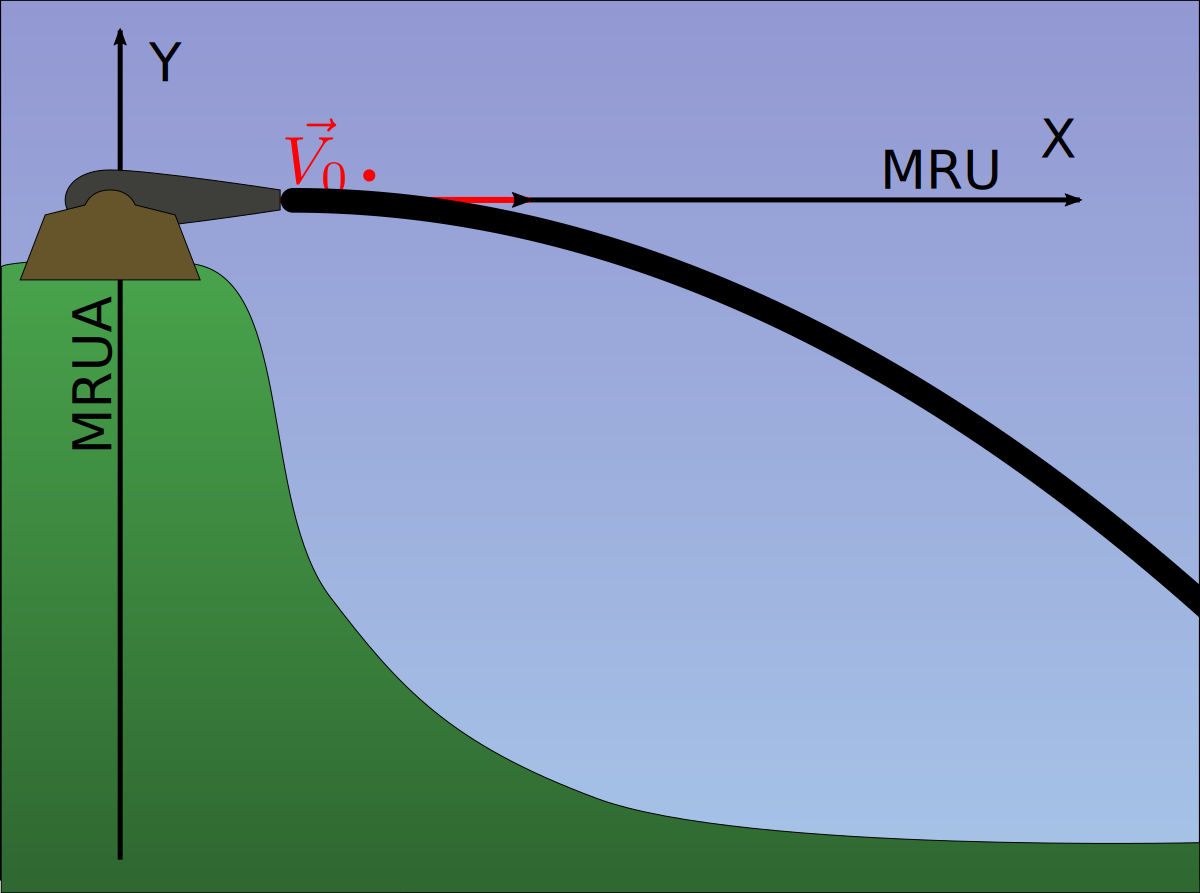
\includegraphics[width=.5 \linewidth]{tir_horizontal.png}
    \caption{Schéma d'un tir horizontal.}
    \label{Schéma d'un tir horizontal}
\end{figure}

\section{Indépendance des mouvements en deux dimensions}
La photo ci-dessous est une chronophotographie présentant deux corps laissés en chute libre au même instant. Celui de gauche possède une vitesse en X non nulle, il s'agit donc d'un tir horizontal.
\begin{figure}[h!]
    \centering
    \includegraphics[width=.5 \linewidth]{chronophoto_tir_horizontal.jpg}
    \caption{Chronophotographie d'un tir horizontal comparé à une chute libre.}
    \label{chronophoto_tir_horizontal}
\end{figure}
Cette image montre que les deux corps tombent en même temps, la seule différence est que celui de gauche avance en même temps qu'il tombe.


\begin{encadre}
    Dans un mouvement à deux dimensions, le mouvement horizontal est totalement indépendant du mouvement vertical. Le mouvement vertical est celui d'une chute libre : un MRUA causé par l'accélération de la pesanteur terrestre.
    L'accélération étant uniquement dirigée vers le bas, le mouvement horizontal du corps est celui d'un MRU.
\end{encadre}

\newpage

\section{Le vecteur vitesse dans un mouvement à deux dimensions}
À un moment donné de sa trajectoire, le mobile possède à la fois une vitesse horizontale, \(\vec{v_x}\), et une vitesse verticale, \(\vec{v_y}\). La vitesse totale du mobile à un instant quelconque est donc donnée par la somme vectorielle de la vitesse horizontale et de la vitesse verticale. Cette somme se fait en utilisant le théorème de Pythagore : \(v_{tot}=\sqrt{v_x ^2 + v_y ^2}\)

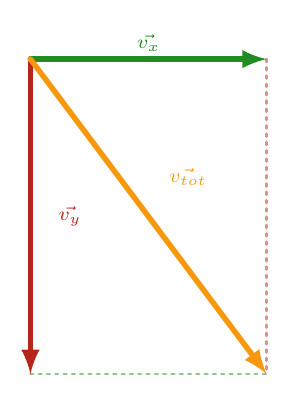
\begin{tikzpicture}[line cap=round,line join=round]
    \tikzset{>=latex}

    \draw [line width=1pt,color=ForestGreen,style=dotted,draw opacity=0.5] (0,-4) -- (3,-4);
    \draw [line width=1pt,color=BrickRed,style=dotted,draw opacity=0.5] (3,0) -- (3,-4);

    \draw [->,line width=2pt,color=BrickRed] (0,0) -- (0,-4);
    \draw [->,line width=2pt,color=ForestGreen] (0,0) -- (3,0);
    \draw [->,line width=2pt,color=YellowOrange] (0,0) -- (3,-4);

    \begin{scriptsize}
        \draw[color=BrickRed] (0.5,-2) node {\(\vec{v_y}\)};
        \draw[color=ForestGreen] (1.5,0.2) node {\(\vec{v_x}\)};
        \draw[color=YellowOrange] (2,-1.5) node {\(\vec{v_{tot}}\)};
    \end{scriptsize}
\end{tikzpicture}

\section{Exercices}
\begin{exercise}
    Un objet est lancé horizontalement depuis une hauteur de \(6\unit{[m]}\) et avec une vitesse de \(4\unit{[m/s]}\).
    \begin{enumerate}[label=\alph*)]
        \item Combien de temps prend-il pour atteindre le sol ?
        \item Quelle distance parcoure-t-il horizontalement avant de toucher le sol ?
        \item Quelle est sa vitesse totale à l'impact ?
    \end{enumerate}
\end{exercise}

\begin{exercise}
    Quelle doit être la vitesse initiale d'un projectile lancé horizontalement depuis une hauteur de \(25[m]\) pour qu'il atteigne le sol à une distance horizontale de \(40[m]\) par rapport à sa position de départ ?

    Quelle sera sa vitesse totale à l'impact ?
\end{exercise}

\begin{exercise}
    Un objet est lancé horizontalement avec une vitesse de \(15\unit{[m/s]}\). Il touche le sol avec une vitesse totale d'impact de \(55\unit{[m/s]}\). De quelle hauteur a-t-il été lâché ?
\end{exercise}
\begin{solution}
    \(v_{y ; impact}=-52,92\unit{[m/s]}\)
    \(t_{chute}=5,394\unit{[s]}\)
    \(y_0142,7[m]\)
\end{solution}

\begin{exercise}
    Un objet est lancé horizontalement avec une vitesse de \(10\unit{[m/s]}\). Il touche le sol \(5[m]\) plus loin, en distance horizontale. De quelle hauteur a-t-il été lancé ?
\end{exercise}
\begin{solution}
    \(t_{chute}=0,5\unit{[s]}\)
    \(y_0=1,226[m]\)
\end{solution}

\begin{exercise}
    Un objet est lancé horizontalement. Il touche le sol \(5\unit{[s]}\) plus tard et \(10[m]\) plus loin.
    \begin{enumerate}[label=\alph*)]
        \item De quelle hauteur a-t-il été lancé ?
        \item Quelle est sa vitesse totale à l'impact ?
    \end{enumerate}
\end{exercise}
\begin{solution}
    \(y_0=122,6[m]\)
    \(v_x=2\unit{[m/s]}\)
    \(v_{y;impact}=-49,05\unit{[m/s]}\)
    \(v_{impact}=49,09\unit{[m/s]}\)
\end{solution}
